\section{在 Linux 系统上编译和运行 CUDA 程序}

本章讲解如何在 Linux 系统上编译和运行 CUDA 程序。请先阅读前一章的内容，因为本章不再重复解释相同的项目。

打开包含本章所有项目的文件夹，使用任意编辑器打开第一个项目 \texttt{project\_01}。例如，使用 Visual Studio Code 打开后，
可以看到一个 GPU 核函数，用于打印块 ID、线程 ID 和 Warp ID。我们使用两个块，每个块包含 64 个线程来启动该核函数。

\subsection{使用 nvcc 编译}

Visual Studio Code 本身只是编辑器，不具备编译功能。需要打开命令提示符，输入 \texttt{wsl} 在 Windows 上启动 Linux 子
系统（安装方法详见前文章节），然后进入项目文件夹。

使用 \texttt{nvcc --version} 可以检查 nvcc 编译器是否已安装。编译命令如下：

\begin{verbatim}
nvcc -o project_01 project_01.cu
\end{verbatim}

其中 \texttt{-o} 用于指定可执行文件的名称（建议在所有编译命令中都使用它）。编译完成后，输入 \texttt{ls} 即可看到生成的
可执行文件。

\subsection{运行程序与输出问题}

运行程序时，输入 \texttt{./project\_01} 并按回车。但有时终端上没有任何输出——项目本应为每个线程打印一行内容。

\begin{figure}
    \centering
    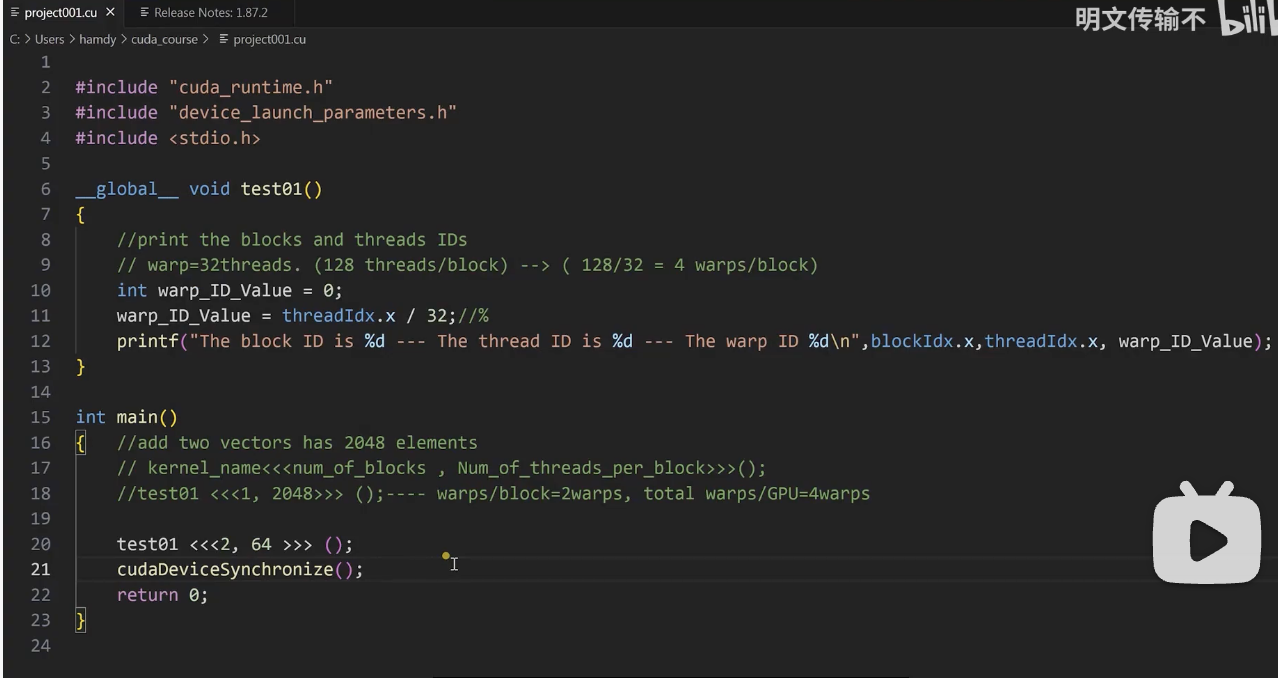
\includegraphics[width=0.75\linewidth]{resources/cuda-071.png}
    \caption{}
    \label{fig:placeholder}
\end{figure}

再运行一次，这次有输出了。程序本身没有问题，但第一次运行时终端上缺少输出，这是怎么回事？

\subsection{cudaDeviceSynchronize}

原因在于 CPU 与 GPU 的执行是异步的。在 CPU 一侧，主函数会逐条执行指令。当遇到启动 GPU 核函数的指令时，CPU 会将
核函数发送到 GPU，但不会等待 GPU 的执行结果，而是立即执行下一条指令。因此，GPU 的 \texttt{printf} 输出可能来不
及在程序结束前显示。

解决方案是使用 \texttt{cudaDeviceSynchronize()}——"同步"意味着让 CPU 等待，直到 GPU 完成核函数的执行。在核函数
调用之后添加这一行：

\begin{verbatim}
kernel<<<blocks, threads>>>();
cudaDeviceSynchronize();
\end{verbatim}

编译并运行后，每次都能看到完整的输出。不使用 \texttt{cudaDeviceSynchronize()} 时，输出时有时无；使用后则始终
稳定输出。

这一同步机制不仅适用于 Linux，也适用于 Windows。

\subsection{编译错误排查}

如果故意制造编译错误（例如删除某个分号），编译器会提示错误出现在某一行。需要注意的是：分号缺失通常会反映在下一条指令
上，因此应检查报错行的上一条语句。修正错误后保存并重新编译即可。

以上就是在 Linux 系统上编译和运行 CUDA 应用程序的完整流程。

